%%%%%%%%%%%%%%%%%%%%%%%%%%%%%%%%%%%%%%%%%%%%%%%%%%%%%%%%%%%%%%
%% LaTeX template for the science justification to be       %%
%%     submitted as part of a regular ALMA proposal.        %%
%% This template should also be used for a ToO, DDT, or     %%
%%     mm-VLBI ALMA proposal, but NOT for Large Programs    %%
%%     (these have a separate template with more sections)  %%
%%                                                          %%
%%                      ALMA Cycle 9                        %%
%%                                                          %%
%%%%%%%%%%%%%%%%%%%%%%%%%%%%%%%%%%%%%%%%%%%%%%%%%%%%%%%%%%%%%%

%%%%%%%%%%%%%%%%%%%%%%%%%%%%%%%%%%%%%%%%%%%%%%%%%%
%%%%% How to convert this document to PDF %%%%%%%%
%%%%%%%%%%%%%%%%%%%%%%%%%%%%%%%%%%%%%%%%%%%%%%%%%%

% If your figures are stored as PostScript files, you can use the 
% following commands to generate a PDF file of your proposal:

%% latex file.tex
%% dvips file.dvi
%% ps2pdf file.ps file.pdf 


% If your figures are PDF images or bitmap pictures in PNG, JPG, or GIF format,
% you can use the pdflatex command to generate a PDF file from this template
% (note, however, that the pdflatex command does not handle PostScript files):

% pdflatex file.tex

% Warnings: 
%           1. You must make sure that PDF output generated from this
%              template is complete both when displayed with a viewer 
%              (acroread, for example) and when printed on paper.
%              LaTeX installations vary greatly and therefore it might 
%              not be possible to get all proposals to come out 
%              correctly with a single text page layout. 
%              In some cases you will have to adjust the 
%              \topmargin=-7mm command in the template to center the 
%              text vertically in the page.  
%           2. The scientific justification, figures, tables, references,
%              and public outreach statement must all fit within the
%              4-page limit.
%           3. You are free to include colour images in your proposal justification.
%              Proposals are distributed to ALMA Review Panels and to distributed
%              peer review reviewers in electronic form.
%              However, the scientific content of the images should still remain
%              clear when displayed or printed in black and white.
%           4. This template is for regular, ToO, DDT, or mm-VLBI ALMA proposals,
%              but NOT for Large Programs: these have a separate template with
%              more sections, and is available from the ALMA Science Portal


%%%%%%%%%%%%%%%%%%%%%%%%%%%%%%%%%%%%%%%%%%%%%%
%%%%% Default format: 12pt single column %%%%%
%% 12pt is the minimum font size allowed !! %%
%% This applies to everything, including    %%
%% references, figure captions, and tables  %%
%% ==> Proposals not compliant to this will %%
%%     be rejected. See Section 5.3.1 in    %%
%%     the ALMA Proposer's Guide            %%
%%%%%%%%%%%%%%%%%%%%%%%%%%%%%%%%%%%%%%%%%%%%%%

\documentclass[12pt,a4paper]{article}  %% DO NOT CHANGE to 11pt or less !

\usepackage[dvipdfmx]{graphics, graphicx}
% if you on overleaf...
\usepackage{color}
% if you on local...
% \usepackage[dvipdfmx]{color}
\usepackage{amsmath,amssymb}
\usepackage{natbib}
\usepackage{aas_macros}
\usepackage{compactbib}
\usepackage{txfonts}
\usepackage{threeparttable}
\usepackage{xspace}
\usepackage{enumitem}
\usepackage{adjustbox}
\usepackage{wrapfig}
\usepackage[colorlinks=true,citecolor=blue]{hyperref}

\newcommand{\ammonia}{NH$_3$\xspace}

%%%%%%%%%%%%%%%%%%%%%%%%%%%%
%%%%%% Page dimensions %%%%%
%%%%%%  DO NOT CHANGE  %%%%%
%%%%%%%%%%%%%%%%%%%%%%%%%%%%

\textheight=247mm
\textwidth=180mm
\topmargin=-7mm
\oddsidemargin=-10mm
\evensidemargin=-10mm
\parindent 10pt

%%%%%%%%%%%%%%%%%%%%%%%%%%%%%
%%%%% Start of document %%%%% 
%%%%%%%%%%%%%%%%%%%%%%%%%%%%%

\begin{document}
\pagestyle{plain}
\pagenumbering{arabic}
 
% The title, abstract and list of investigators should NOT be included in the
% Scientific justification. The title and abstract are put automatically on the cover page.

%%%%%%%%%%%%%%%%%%%%%%%%%%%%%%%%%%%%%%%%%
%%%%% Body of science justification %%%%%
%%%%%%%%%%%%%%%%%%%%%%%%%%%%%%%%%%%%%%%%%

%% ENTER TEXT, FIGURES AND TABLES BELOW
%% Minimum font size for all text, references, figure captions, and tables is 12pt
%% Proposals not compliant to this will be rejected. See Section 5.3.1 in the ALMA Proposer's Guide.

\section{Scientific Justification}
% Nitrogen is the fifth most abundant elements in the interstellar medium (ISM) with elemental abundances of $\sim6\times10^{-5}$ with respect to hydrogen. 
\subsection{Background}
\noindent \textbf{Nitrogen chemistry} \quad Nitrogen is one of the key elements for the chemistry of star and planet formation. It is the third most abundant heavy element after carbon and oxygen \citep{Przybilla08}. Nitrogen in star-forming clouds is incorporated into planet-forming disks as volatiles such as N$_2$, which also affects disk chemistry \citep[e.g.,][]{Schwarz14}. These volatiles eventually become the building material of planetary bodies. In addition, molecules such as \ammonia that formed in molecular clouds or cloud cores set the initial condition of organic chemistry and its abundance will effectively affect the formation paths and efficiencies of nitrogen-bearing organic molecules in the later stages of star and planet formation.

\smallskip
\noindent In order to understand the nitrogen chemistry in the interstellar medium (ISM), it is essential to determine the primary nitrogen reservoir. Nitrogen chemistry in the ISM consists of three competing processes; conversion from N atoms into N$_2$ molecules via gas-phase reactions, the reverse process (e.g., photodissociation), and the freeze-out of N and N$_2$ onto dust grains followed by surface reactions \citep[e.g.,][]{Daranlot12}. Thus, it is expected that the main nitrogen reservoir is either in molecular (N$_2$) or atomic (N) form, or icy nitrogen-bearing molecules (e.g., \ammonia). However, the main nitrogen reservoir is not yet observationally constrained, and nitrogen chemistry is thus poorly understood. Ice observations with \textit{Spitzer} revealed that only $\sim$10\% of overall nitrogen is locked up into ices as \ammonia, NH$_4^+$, and OCN$^-$ \citep{Oberg11}. Direct observations of N and N$_2$ are difficult in both ice and gas. \citet{Maret06} instead observed N$_2$H$^+$, which is primary formed by N$_2$ + H$_3^+$, to conclude that it is unlikely that the gaseous N$_2$ is the main nitrogen reservoir. %Alternatively, a large fraction of N$_2$ might be locked up into ices. A very uncertain upper limit of N$_2$ ice abundance in molecular clouds have been inferred indirectly to be $\lesssim$40\% of overall nitrogen \citep{Boogert15}. 
%Furthermore, in situ measurements on the comet 67P/Churyumov-Gerasimenko by the Rosetta mission suggested that a substantial amount of nitrogen is hidden as ammonium salts \citep{Altwegg20}.

\medskip
\noindent \textbf{Deuteration of ammonia ice} \quad  %It is well established that deuterium enrichment is sensitive to various physical and chemical conditions and thus used to probe the formation stage of molecules \citep[e.g.,][]{Ceccarelli14}. 
It is well established that the deuteration sensitively depends on various physical and chemical conditions. In  molecular clouds, where the density and visual extinction are relatively low ($n\sim10^{3}$--10$^{4}$\,cm$^3$), the molecular D/H ratios are lower ($\sim$10$^{-3}$--10$^{-4}$), while it will be higher in dense cores (or prestellar cores) due to their cold ($\lesssim$20\,K) and dense ($\gtrsim$10$^5$\,cm$^{-3}$) environment and the freeze-out of CO. As the D/H ratios of icy molecules are determined when they form and do not change significantly later, they contain the information about the formation stage of the molecules. Thus, if the bulk ammonia ices have formed in molecular clouds (i.e., the main nitrogen reservoir is molecular form), the ice abundance ratio of NH$_2$D/NH$_3$ ($=f_\mathrm{D1}$) will be lower. On the other hand, if the ammonia ices are mainly formed in dense cores (i.e., the atomic nitrogen remains as the main nitrogen reservoir) 

Since the ammonia ices are formed by the sequential addition of H (or D) to the N atom, 


% \citet{Furuya18} proposed a new approach to constrain the main nitrogen reservoir using multiply-deuterated ammonia ice. The ammonia ice, NX$_3$, where X is H or D, are mainly formed by sequential hydrogenation of \textit{atomic nitrogen} on the dust grain surfaces in molecular clouds or dense cores. 
% In molecular clouds, their relatively high temperature ($\gtrsim$20\,K) and low density ($\sim$10$^3$--10$^4$\,cm$^{-3}$) will result in a lower D/H ratio ($\sim$10$^{-3}$--10$^{-4}$), while it will be higher in dense cores (or prestellar cores) due to their cold ($\lesssim$20\,K) and dense ($\gtrsim$10$^5$\,cm$^{-3}$) environment and the freeze-out of CO.
% In molecular clouds, where density is $\sim$10$^3$--10$^4$\,cm$^{-3}$, the molecular D/H ratios are lower ($\sim$10$^{-3}$--10$^{-4}$), while it will be higher in dense cores (or prestellar cores) due to their cold ($\lesssim$20\,K) and dense ($\gtrsim$10$^5$\,cm$^{-3}$) environment and the freeze-out of CO.
%In particular, the abundance ratios such as NHD$_2$/NH$_2$D ($=f_\mathrm{D2}$) and ND$_3$/NHD$_2$ ($=f_\mathrm{D3}$) selectively reflect the deuteration in dense cores over the NH$_2$D/NH$_3$ ($=f_\mathrm{D1}$) because multiply-deuterated ammonia ices are mostly formed in the dense core stage where the deuteration is particularly efficient. Thus, if the atomic nitrogen (ingredient of ammonia ice) is the main nitrogen reservoir and ammonia ices are mainly formed in dense cores, $f_\mathrm{D2}$ and $f_\mathrm{D3}$ will be lower than $f_\mathrm{D1}$ and $f_\mathrm{D2}$, respectively (the right panel of Figure \ref{fig:ammonia_deuteration}). On the other hand, if the atomic nitrogen is largely converted into the stable molecular form (i.e., N$_2$ and NH$_3$) in molecular clouds and the formation of ammonia ices continues with a reduced efficiency in dense cores, $f_\mathrm{D2}$ and $f_\mathrm{D3}$ should be comparable to or larger than $f_\mathrm{D1}$ and $f_\mathrm{D2}$, respectively (the left panel of Figure \ref{fig:ammonia_deuteration}).  
The abundance ratios of NHD$_2$/NH$_2$D ($=f_\mathrm{D2}$) selectively reflect the deuteration in dense cores over the NH$_2$D/NH$_3$ ($=f_\mathrm{D1}$) because doubly-deuterated ammonia ices are mostly formed in the dense core stage where the deuteration is particularly efficient. 
Thus, if the atomic nitrogen is largely converted into the stable molecular form (i.e., N$_2$ and NH$_3$) in molecular clouds and the formation of ammonia ices continues with a reduced efficiency in dense cores, $f_\mathrm{D2}$ should be larger than $f_\mathrm{D1}$ (the left panel of Figure \ref{fig:ammonia_deuteration}). On the other hand, if the atomic nitrogen (ingredient of ammonia ice) is the main nitrogen reservoir and ammonia ices are mainly formed in dense cores, $f_\mathrm{D2}/f_\mathrm{D1}$ will be close to the statistical value (1/3) and $f_\mathrm{D2}$ will be lower than $f_\mathrm{D1}$ (the right panel of Figure \ref{fig:ammonia_deuteration}).
% Thus, if the atomic nitrogen (ingredient of ammonia ice) is the main nitrogen reservoir and ammonia ices are mainly formed in dense cores, $f_\mathrm{D2}/f_\mathrm{D1}$ will be close to the statistical value (1/3) and $f_\mathrm{D2}$ will be lower than $f_\mathrm{D1}$ (the right panel of Figure \ref{fig:ammonia_deuteration}). On the other hand, if the atomic nitrogen is largely converted into the stable molecular form (i.e., N$_2$ and NH$_3$) in molecular clouds and the formation of ammonia ices continues with a reduced efficiency in dense cores, $f_\mathrm{D2}$ should be comparable to or larger than $f_\mathrm{D1}$ (the left panel of Figure \ref{fig:ammonia_deuteration}). 
A similar relation should be hold between ND$_3$/NHD$_2$ ($=f_\mathrm{D3}$) and $f_\mathrm{D2}$ as well. \citet{Furuya18} quantitatively confirmed these scenarios by conducting the gas-ice astrochemical simulation from the formation of molecular clouds to the protostellar core stage with different initial nitrogen partitions (Table \ref{tab:model}). Indeed, the two models present a striking contrast: while the molecule dominant model shows $f_\mathrm{D1} \ll f_\mathrm{D2} \approx f_\mathrm{D3}$, for the atom dominant model $f_\mathrm{D1} > f_\mathrm{D2} > f_\mathrm{D3}$ is satisfied.

\vspace{-1.2em}
\begin{center}
\begin{threeparttable}[tbh]
\caption[]{Ammonia deuteration in the hot corino region in the model by \citet{Furuya18}}
\begin{tabular}{lcccccc}
\hline \noalign {\smallskip}
Model  & Atomic N (\%) & N$_2$ (\%) & NH$_3$ (\%) & $\frac{\mathrm{NH_2D}}{\mathrm{NH_3}}\,(f_\mathrm{D1})$ & $\frac{\mathrm{NHD_2}}{\mathrm{NH_2D}}\,(f_\mathrm{D2})$ &
$\frac{\mathrm{ND_3}}{\mathrm{NHD_2}}\,(f_\mathrm{D3})$\\
\hline \noalign {\smallskip}
Molecule dominant & 0.051 & 22 & 76 & 0.004 & 0.018 & 0.017 \\
Atom dominant & 57 & 13 & 28 & 0.020 & 0.013 & 0.006 \\
\hline \noalign {\smallskip}
\end{tabular}
\label{tab:model}
\end{threeparttable}
\end{center}
\vspace{-0.5em}


% the D/H ratio of ammonia ices will be high (a few percent or higher) and the ratios such as [ND$_3$/NHD$_2$]/[NHD$_2$/NH$_2$D] and [NHD$_2$/NH$_2$D]/[NH$_2$D/NH$_3$] are close to the statistical value (1/3) and lower than unity. On the other hand, if the atomic N is largely converted into the stable molecular form (i.e., N$_2$ and NH$_3$) in molecular clouds, the ratios should be larger than unity. 

\begin{figure}[th]
    \centering
    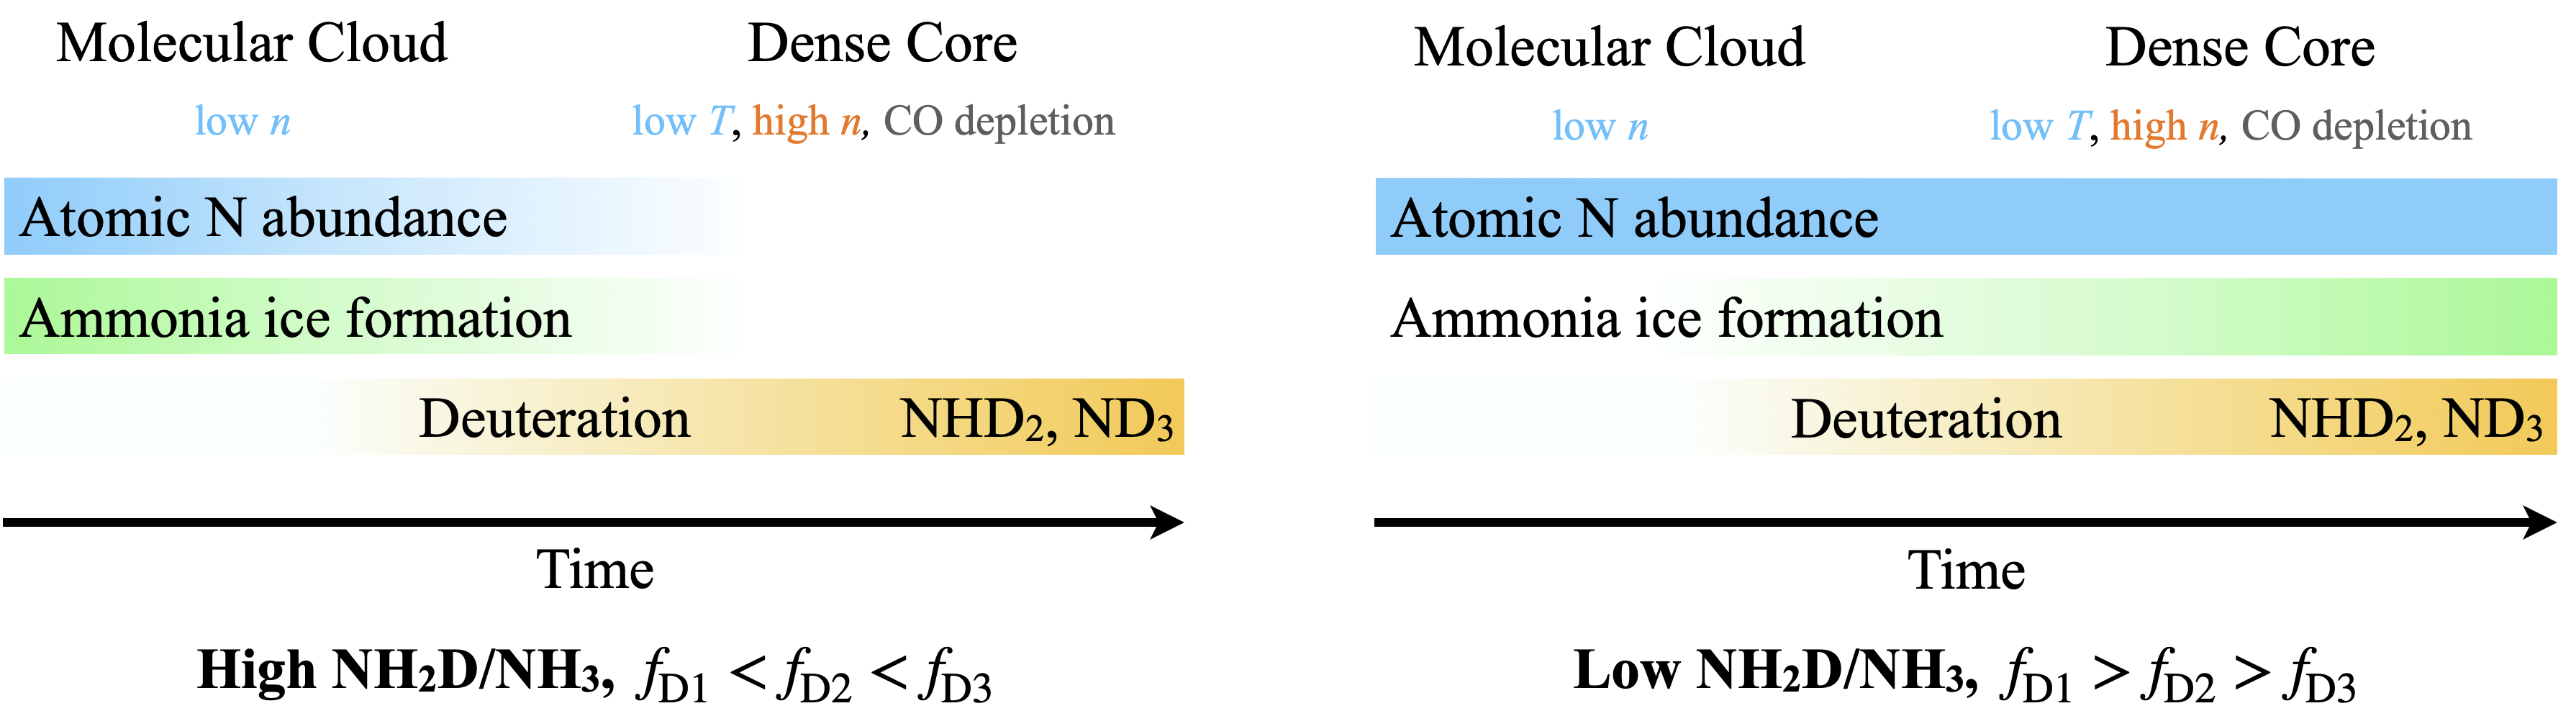
\includegraphics[width=\textwidth]{ammonia_deuteration_cartoon_no_schemfig_ver2.png}
    \caption{Relation between the main nitrogen reservoir and deuteration of ammonia ices. \textit{left:} In the case that the atomic nitrogen has been mostly converted into molecules in dense cores. This will result in the $f_\mathrm{D3}$/$f_\mathrm{D2}$ and $f_\mathrm{D2}$/$f_\mathrm{D1}$ ratios of higher than unity. \textit{right:} In the case that the atomic nitrogen remains as the main nitrogen reservoir in dense cores. The $f_\mathrm{D3}$/$f_\mathrm{D2}$ and $f_\mathrm{D2}$/$f_\mathrm{D1}$ ratios will present the statistical values and will be lower than unity.}
    \label{fig:ammonia_deuteration}
\end{figure}

\smallskip
\noindent The best and only way to measure the D/H ratios of ammonia ices is to observe the fresh ammonia gas that have just sublimated from the dust grain surfaces in the inner warm (typically $\lesssim$100\,au and $T\gtrsim100$\,K) region of the protostellar envelopes, so-called \textit{hot corinos}. \textbf{Here, we propose to observe NH$_2$D, NHD$_2$, and ND$_3$ molecular lines at $\sim$300\,GHz to measure the D/H ratios of ammonia ices toward multiple hot corinos, taking advantage of the high resolution and high sensitivity of ALMA. This will reveal the main nitrogen reservoir in star-forming clouds and will be the crucial first step to elucidate nitrogen chemistry in the ISM.}

\subsection{Previous Observations of Deuteration in Hot Corinos}
% Surprisingly, recent observations with the Karl G. Jansky Very Large Array (VLA) found an extremely high D/H ratio of $f_\mathrm{D1}\sim0.5$--1 toward the hot corinos of the protobinary NGC1333 IRAS4A (Figure \ref{fig:IRAS4A_VLA}, article in preparation). 

% This is even higher than the value in the atom dominant model \cite[0.02;][]{Furuya18} by orders of magnitude.     

So far, observations of the deuteration for several abundant molecules toward hot corinos have been reported. The D/H ratios of water (HDO/H$_2$O) have been revealed to be relatively low \citep[$\sim$10$^{-3}$--10$^{-4}$; e.g.,][]{Jorgensen10}, while those of methanol (CH$_3$OD/CH$_3$OH, CH$_2$DOH/CH$_3$OH) are higher \citep[$\sim$10$^{-2}$; e.g.,][]{Bianchi17}. This contrast suggests that water ices are formed mainly in molecular clouds, followed by the formation of methanol ices in the later evolutionary stage (i.e., molecular cloud core). The astrochemical model presented in \citet{Furuya18} have also supported this picture. 

\begin{wrapfigure}[13]{r}[0\hsize]{0.55\hsize}
\centering
\vspace{-1em}
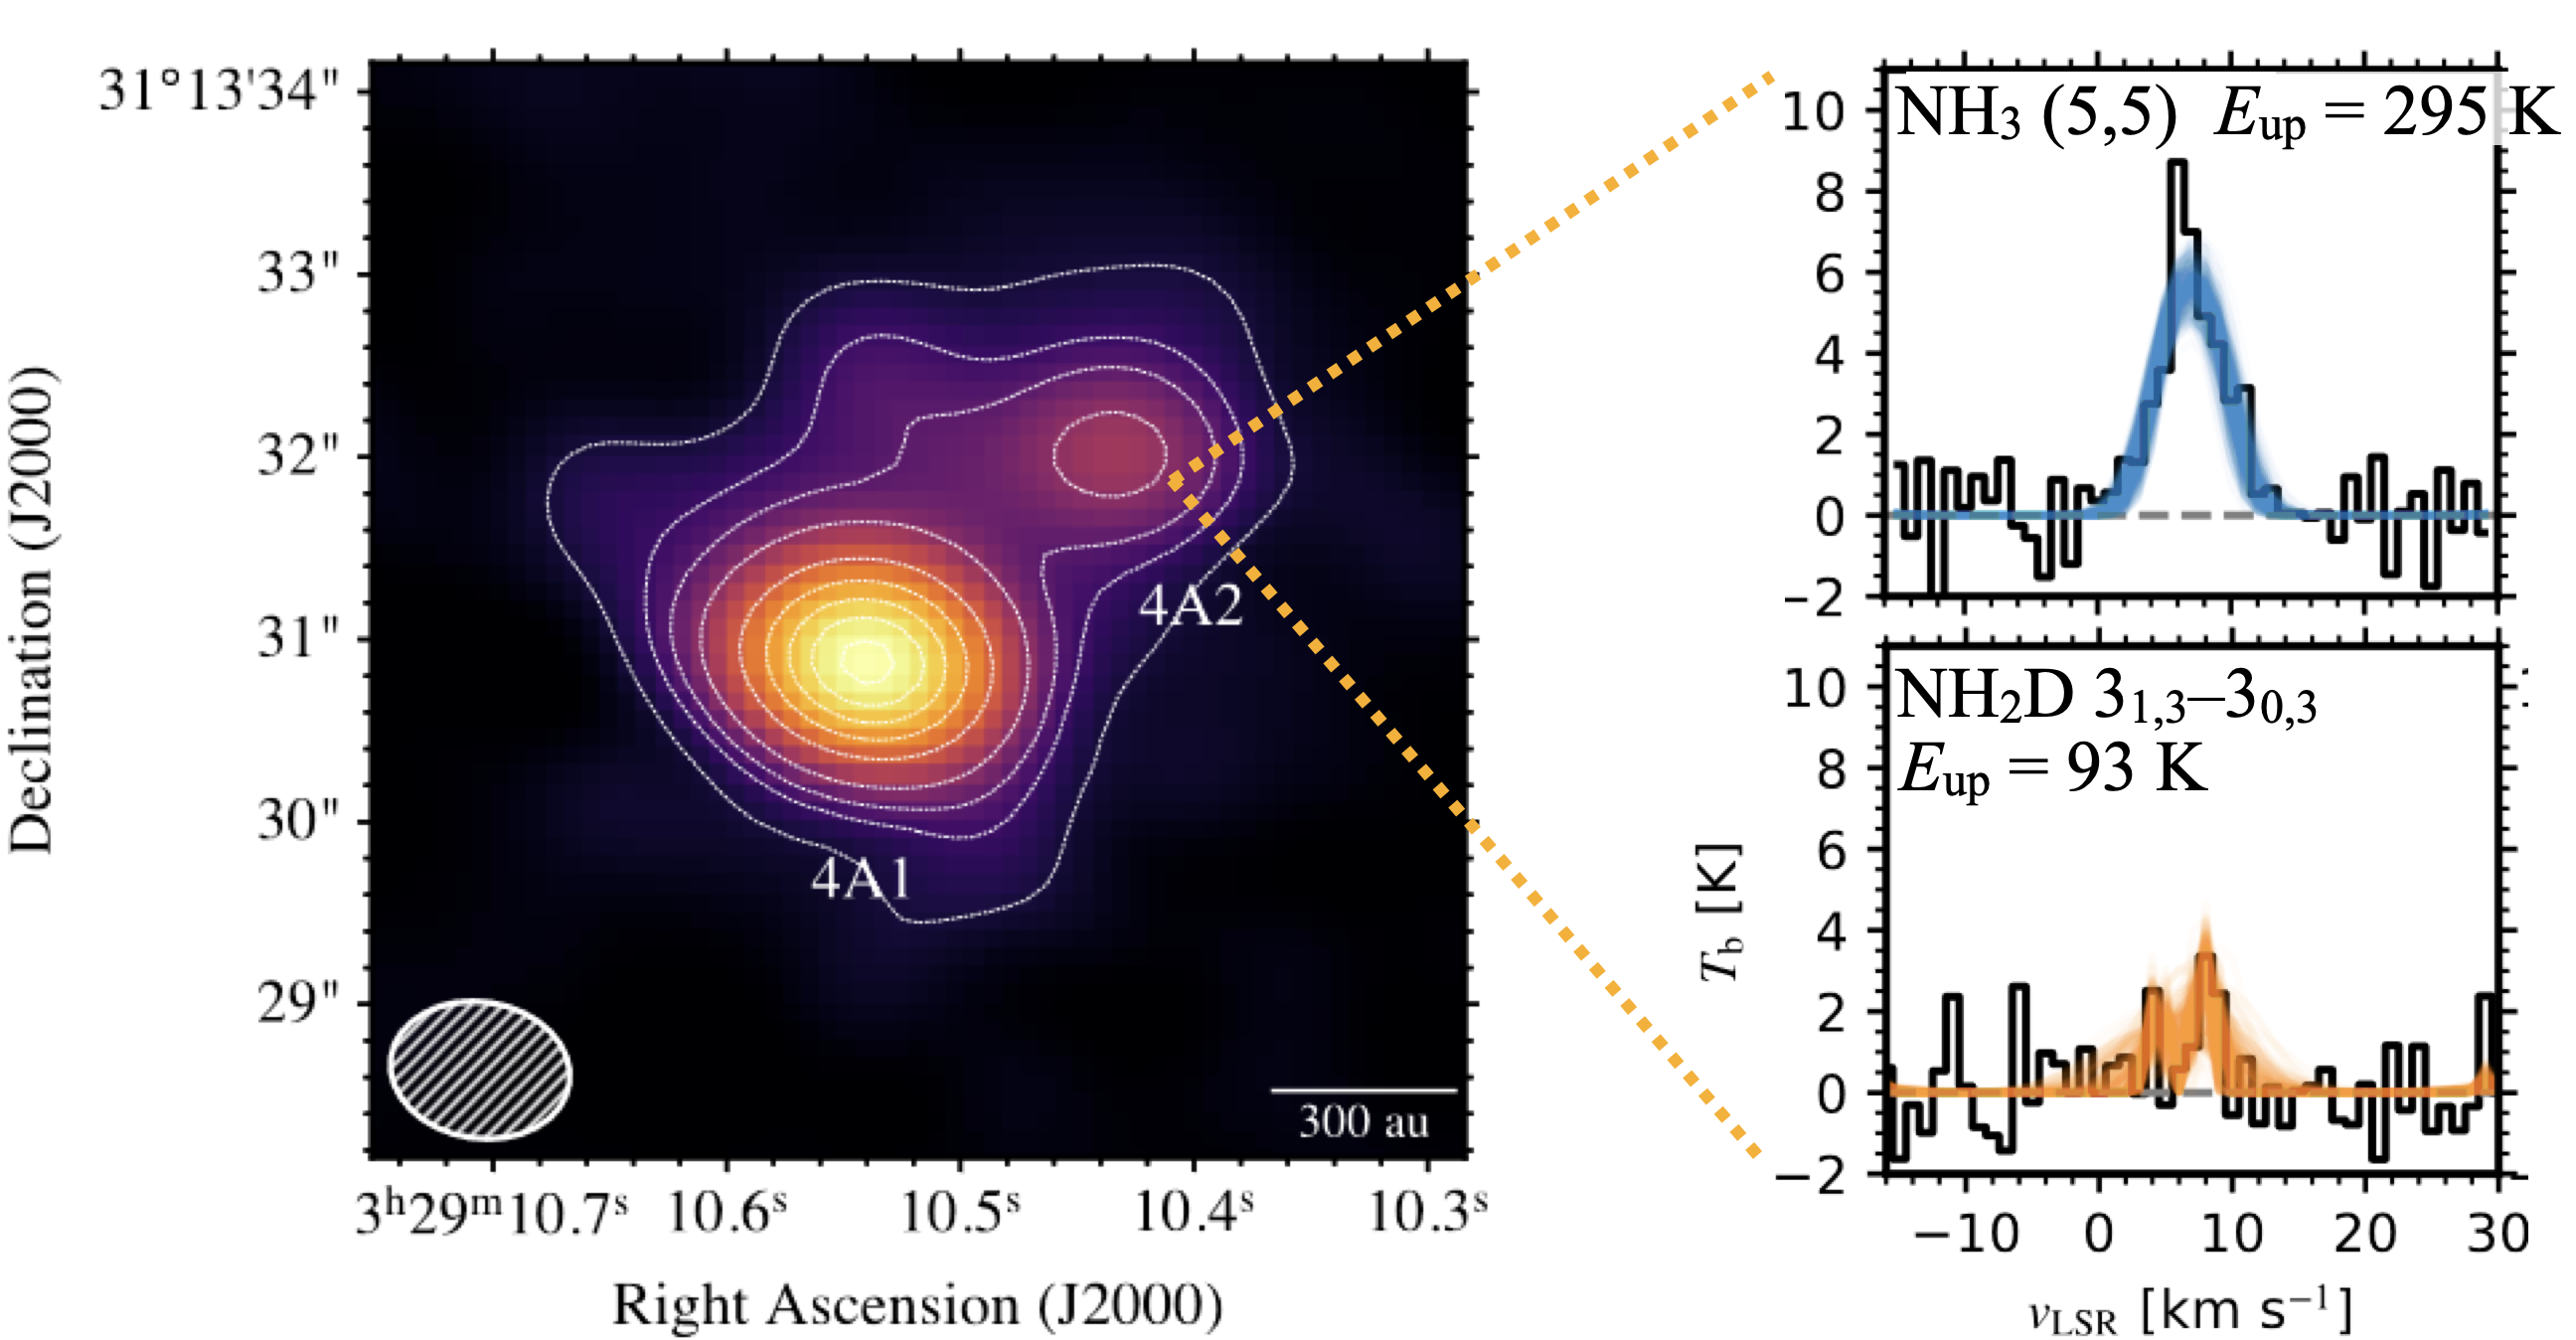
\includegraphics[keepaspectratio, width=0.95\hsize]{IRAS4A_ammonia.png}
\caption{VLA observations of continuum (left) and NH$_3$ and NH$_2$D spectra (right) toward NGC1333 IRAS4A.}
\label{fig:IRAS4A_VLA}
\end{wrapfigure}

\smallskip
\noindent Recent observations with the Karl G. Jansky Very Large Array (VLA) have detected the multiple \ammonia and NH$_2$D lines toward the hot corinos of the protobinary NGC1333~IRAS4A (Figure \ref{fig:IRAS4A_VLA}, article in preparation), and the $f_\mathrm{D1}$ abundance ratio has been constrained for the first time in hot corinos. Surprisingly, the ratio is extremely high ($\sim$0.5--1) and even higher than the value in the atom dominant model (Table \ref{tab:model}). This possibly suggests that ammonia ices are formed in the later evolutionary stage than methanol ices, and that the atomic nitrogen still remains as the main nitrogen reservoir in that stage. On the other hand, there are still possibilities that the VLA observations of the NH$_2$D line trace the more extended region than the NH$_3$ line within the observed beam ($\sim$1\arcsec or $\sim$300\,au), as indicated by the narrower line width and lower excitation energy of the NH$_2$D line (see the spectra in Figure \ref{fig:IRAS4A_VLA}). This might be the cause of the extremely high $f_\mathrm{D1}$ ratio as the D/H ratios are expected to be higher in the outer region \citep{Furuya18}. Observations with higher angular resolutions are needed to selectively trace the innermost region where ammonia ices have fully sublimated. Also, the VLA observations are just the first attempt to constrain the D/H ratios of ammonia ices and the main nitrogen reservoir. Further observations of deuterated ammonia lines toward another source are needed to confirm that the high D/H ratios of ammonia is common. 



%The high excitation energies of the lines observed ($\gtrsim$100\,K) and small emitting region size ($\sim$100\,au) derived from the line profile fit indicate that the observed line emission originates from the inner warm region where the ammonia ices have fleshly sublimated. Thus, 
% The high $f_\mathrm{D1}$ ratio possibly suggests that the ammonia ices are mainly formed in the dense core stage and the atomic nitrogen still remains as the main nitrogen reservoir in that stage. However, these observations did not constrain $f_\mathrm{D2}$ or $f_\mathrm{D3}$, which are essential for robustly claiming the main nitrogen reservoir, and are just the first attempt to constrain the main nitrogen reservoir.


%\citet{Jorgensen10} have found a low HDO/H$_2$O abundance ratio of $\lesssim6 \times 10^{-4}$ for the first time toward the hot corino in NGC1333 IRAS4B. 
% \citet{Coutens14} have observed the doubly-deuterated water (D$_2$O) toward another hot corino in NGC1333 IRAS2A to find a higher D$_2$O/HDO ratio than HDO/H$_2$O ratio by about one order of magnitude. This has been interpreted as follows: the formation of water ices started in molecular clouds, which resulted in the low HDO/H$_2$O ratio, and continued with a reduced efficiency in dense cores as reflected in the relatively high D$_2$O/HDO ratio \citep{Furuya16}. This work demonstrated that the multiply-deuterated specie can be a powerful tool to trace the formation history of molecules.

% \smallskip



% \noindent Recent observations with the Karl G. Jansky Very Large Array (VLA) have detected the multiple \ammonia and NH$_2$D lines toward the hot corinos of the protobinary NGC1333~IRAS4A (Figure \ref{fig:IRAS4A_VLA}, private communication). The $f_\mathrm{D1}$ column density ratio has been constrained for the first time in hot corinos to be $\sim$0.5--1 by employing the line profile fit. %The high excitation energies of the lines observed ($\gtrsim$100\,K) and small emitting region size ($\sim$100\,au) derived from the line profile fit indicate that the observed line emission originates from the inner warm region where the ammonia ices have fleshly sublimated. Thus, 
% The high $f_\mathrm{D1}$ ratio possibly suggests that the ammonia ices are mainly formed in the dense core stage and the atomic nitrogen still remains as the main nitrogen reservoir in that stage. However, these observations did not constrain $f_\mathrm{D2}$ or $f_\mathrm{D3}$, which are essential for robustly claiming the main nitrogen reservoir, and are just the first attempt to constrain the main nitrogen reservoir. 

\subsection{Proposed Observations}
We propose to observe multiple NH$_2$D, NHD$_2$, and ND$_3$ lines in Band 7 toward two hot corinos, NGC1333 IRAS4A2 and IRAS 16293-2422 A, with high angular resolutions of 0\farcs3 and 0\farcs5, respectively. Our primary goals are followings:

\begin{enumerate}[leftmargin=*]
    \setlength\itemsep{-0.2em}
    
    \item[1.] to \textbf{measure the $f_\mathrm{D2}$ and $f_\mathrm{D3}$ abundance ratios toward two hot corinos} by high angular resolution observations of deuterated ammonia lines.
    
    \item[2.] to \textbf{constrain the main nitrogen reservoir in the ISM} by comparing the observed relation between $f_\mathrm{D2}$ and $f_\mathrm{D3}$ abundance ratios and model values in Table \ref{tab:model}.
    
    % \item[1.] to \textbf{constrain the $f_\mathrm{D1}$ and $f_\mathrm{D2}$ abundance ratios toward the hot corino NGC1333 IRAS4A2} in combination with the previous VLA observations.
    % \item[2.] to \textbf{double the sources with known main nitrogen reservoir} in the parental cloud by constraining $f_\mathrm{D2}$ and $f_\mathrm{D3}$ abundance ratio toward another hot corino IRAS 16293-2422 A.
    % \item[2.] to \textbf{confirm that the high D/H ratios of NH$_3$ is common} by constraining $f_\mathrm{D2}$ and $f_\mathrm{D3}$ abundance ratio toward another hot corino IRAS 16293-2422 A.
\end{enumerate}


% (1) to \textbf{constrain the $f_\mathrm{D1}$ and $f_\mathrm{D2}$ abundance ratio toward the hot corino NGC1333 IRAS4A2} in combination with the previous VLA observations, and (2) to \textbf{double the sources with known main nitrogen reservoir in the parental cloud} by constraining $f_\mathrm{D2}$ and $f_\mathrm{D3}$ ratio toward another hot corino IRAS 16293-2422 A.


% constrain $f_\mathrm{D3}/f_\mathrm{D2}$ ratio observe another hot corino IRAS~16293-2422~A to constrain the 
% Our primary goal is to constrain the abundance ratio of $f_2/f_1$ or $f_2$, column density ratio toward hot corinos by detecting NH$_2$D, NHD$_2$ and ND$_3$ transitions in Band 7 to constrain the main nitrogen reservoir in star-forming clouds. 

\medskip
\noindent \textbf{Target sources and lines} \quad NGC1333 IRAS4A2 (hereafter IRAS4A2) and IRAS 16293-2422 A (hereafter I16293A) are well-studied sources in the Perseus star-forming complex \citep[$\sim$300\,pc;][]{Zucker18} and the $\rho$ Ophiucus star-forming region \citep[$\sim$140\,pc;][]{Dzib18}, respectively. Both sources are hot corinos as indicated by the emission of various complex organic molecules (COMs).
% Both sources present the emission of various complex organic molecules (COMs), whose sublimation temperatures ($\sim$100\,K) are similar to ammonia and water, in their hot corinos. 
% The abundances of COMs as well as their isotopic ratios have been inferred \citep[e.g.,][]{Lopez-Sepulcre17, Manigand20}. 
Among the known hot corinos, these sources show the highest column densities of abundant volatiles (e.g., $N$(H$_2$O)$\,\sim\,$10$^{19}$--10$^{20}$\,cm$^{-2}$), which makes these sources most promising to detect weak deuterated ammonia lines assuming the standard abundance ratio in the ISM (e.g., NH$_3$/H$_2$O$\sim$0.05) and probe the inner warm region where ammonia ices have fully sublimated ($\sim$0\farcs3--0\farcs5) with a sufficient angular resolution within a reasonable integration time. 
% For IRAS4A2, %it is difficult to detect the ND$_3$ line with a sufficient angular resolution due to the larger distance; instead, the ancillary data from previous VLA observations of NH$_3$ and NH$_2$D lines helps constrain the main nitrogen reservoir. 
Thus, these sources are the best and ideal target for constraining the main nitrogen reservoir.

\smallskip
\noindent The ALMA Band 7 provides an unique opportunity to observe the multiply-deuterated ammonia lines at $\sim$300\,GHz. In particular, the ND$_3$ lines, which is important to constrain $f_\mathrm{D3}$ abundance ratio, are detectable only at this frequency within reasonable integration time. While the most abundant isotopologue, \ammonia (and $^{15}$NH$_3$ as well), are not observable with ALMA and VLA can observe it, the NHD$_2$ and ND$_3$ lines are detectable only with ALMA at high angular resolution \citep{Furuya18}.    


% \medskip
% \noindent \textbf{Target sources} \quad We propose to observe two sources, IRAS~16293-2422 and NGC1333~IRAS4A, located at the $\rho$ Ophiucus star-forming region \citep[$\sim$140\,pc;][]{Dzib18} and the Perseus star-forming complex \citep[$\sim$300\,pc;][]{Zucker18}, respectively. Both sources are deeply embedded Class~0 protobinaries, and each of the binaries harbors a hot corino. Previous observations and the justification of these sources are described below.

% \begin{itemize}[leftmargin=*]
%     \setlength\itemsep{-0.2em}
    
%     \item IRAS~16293-2422 -- This source has been extensively studied mainly by the ALMA Protostellar Interferometric Line Survey \citep[PILS;][]{Jorgensen16}. Both sources of the binary (IRAS~16293~A and IRAS~16293~B) show the various complex organic molecule (COM) emission in the vicinity of the protostar. The isotopic ratios have been inferred for various molecules \citep{Jorgensen18, Manigand20}, which have been compared with the isotopic composition in the comet 67P/Churyumov-Gerasimenko \citep{Drozdovskaya19}. Among the well known hot corinos, IRAS~16293-2422 is the nearest source and shows the highest column densities of abundant volatiles (H$_2$O and CH$_3$OH), which will uniquely and simultaneously allows for resolving the inner warm region ($\lesssim$100\,au or $\sim$0\farcs7) and detecting the weak ND$_3$ line, assuming the standard ISM abundance ratios. Thus, IRAS~16293-2422 is the best and ideal testbed for constraining the main nitrogen reservoir.  
    
%     % While IRAS~16293~B presents the face-on configuration, IRAS~16293~A shows the more inclined structure. Recent higher spatial resolution observations of dust continuum emission with ALMA revealed that IRAS~16293~A itself can be a binary and has a complicated continuum structure.  
    
%     \item NGC1333~IRAS4A -- This source is also a well-studied protobinary, both of which show the COM line emission as revealed by centimeter observations with Karl G. Jansky Very Large Array \citep[VLA;][]{DeSimone20}. Toward the both of the binary (IRAS~4A1 and IRAS~4A2), recent VLA observations of NH$_3$ and NH$_2$D lines revealed high NH$_2$D/NH$_3$ ratios of $\sim$0.5--1 (private communication), which suggests that the main nitrogen reservoir is atomic nitrogen rather than N-bearing molecules. However, confirmation by doubly- and triply-deuterated ammonia that better trace the main nitrogen reservoir is needed. Combining with the ancillary VLA data, this source will allow us to constrain the main nitrogen reservoir in the secondary source.
% \end{itemize}

\smallskip
\noindent \textbf{Analysis methods} \quad We request to observe \emph{multiple, optically thin} NH$_2$D, NHD$_2$, and ND$_3$ lines with different excitation energy levels. This allows us to constrain the column densities of NH$_2$D, NHD$_2$, and ND$_3$ (and the ratios of $f_\mathrm{D2}$ and $f_\mathrm{D3}$) without the temperature assumption. In the case that the all lines originate from the same region (e.g., similar line widths and emitting region sizes), we will employ the standard LTE/non-LTE analysis with a single excitation/kinetic temperature for all transitions (i.e., rotation diagram method for LTE/LVG analysis for non-LTE). If it is not the case, or the line profile is complicated (e.g., asymmetric features due to the infall motion of the gas), we will employ detailed radiative transfer simulations of the hot corinos, which will be compared with observed line profile. As the physical structures for the simulation, we can use the well-established models of IRAS4A2 and I16293A in literature \citep[e.g.,][]{Persson16, Jacobsen18}. %Note that the ND$_3$ 1(0)0,a--0(0)0,s transition at 309.90\,GHz has the hyperfine splitting that could be spectrally resolved, which can be treated by the spectral line fitting by LTE/non-LTE models and could help determine the ND$_3$ abundance with only this transition. 

\smallskip
\noindent \textbf{Comparison with models} \quad The estimated column density ratios will be compared with the predictions of the model presented in \citet{Furuya18} (Table \ref{tab:model}). 
% They conducted the gas-ice astrochemical simulation from the formation of molecular clouds to the protostellar core stage with different initial nitrogen partitions (Table \ref{tab:model}). The two models present a striking contrast: while the molecule dominant model shows $f_\mathrm{D1} \ll f_\mathrm{D2} \approx f_\mathrm{D3}$, $f_\mathrm{D1} > f_\mathrm{D2} > f_\mathrm{D3}$ for the atom dominant model, quantitatively evidencing that ammonia deuteration can trace the main nitrogen reservoir. 
If the observed column density ratios satisfy $f_\mathrm{D2} < f_\mathrm{D3}$, the main nitrogen reservoir would be molecular form and the formation of ammonia ices started in molecular clouds and continues with a reduced efficiency in dense cores. On the other hand, if the observed column density ratios satisfy $f_\mathrm{D2} > f_\mathrm{D3}$, the main nitrogen reservoir would be atomic nitrogen and ammonia ices are mainly formed in dense cores.  










% \color{red}
% Introduction: Importance of nitrogen chemistry, and it is not yet elucidated, deuteration of ammonia ice can trace the ice formation history and nitrogen partitioning...

% Furuya+18 proposed that the ice formation history and information about main nitrogen reservoir are imprinted into the multiply deuterated ammonia ices. [NHD2/NH2D]/[NH2D/NH3] reflects the deuteration levels of different evolutionary stages. Non-statistical ratio of [D2O/HDO]/[HDO/H2O] is explained by the scenario that the H2O ices are formed in the ealier stages mainly and the formation efficiency is reduced in the later dense core stage

% We can measure the ice deuteration by observing the hot gas sublimated from dust grain surface in the vicinity of the protostar (hot corino)

% We already constrained the NH2D/NH3 ratio with VLA toward prototypical hot corino IRAS 4A. High ratio suggests NH3 ice formed in the later dense core and main nitrogen reservoir could be mostly atomic N toward IRAS 4A. 

% However, we need multiply deuterated ammonia to confirm the scenario proposed in Yamato et al. i.e., how is the ND3/NHD2 ratio which will better trace the later stage ice formation? Also, we need additional sources to confirm if this scenario is ubiquitous or not.

% \color{black}



% ALMA uses two systems to review the proposals submitted in the Main Call.
% All proposals requesting less than 50 h on the 12-m Array and all ACA stand-alone proposals requesting less
% than 150 h on the 7-m Array will be reviewed by Distributed peer review (see Section 1.2.1 of the Proposer's Guide).
% All Large Programs will be reviewed by Panels. 
% Additionally, both systems will follow a dual-anonymous procedure, in which the proposers do not know
% who are the reviewers and the reviews do not who are the proposers.
%
% Please refer to the guidelines before writing your proposal:
%     https://almascience.org/proposing/alma-proposal-review/dual-anonymous
%
% In the following part, describe the scientific background of the project,
% pertinent references and previous work relevant to this 
% proposal, together with any figures and tables that you judge necessary
% (use the following two examples as templates, or remove)
% Please do not disclose the name(s) of the proposer(s), and write the proposal in a way
% such that the proposer(s) cannot be identified. 
 
%-----------------------------Figure Start---------------------------

% The 'scale' parameter below allows you to scale the figure so that it fits within the page.
% In this case the figure was scaled to 20% of its original size.
% Note: for .png files one has to use pdflatex, not classic latex
%
% Minimum font size for references: 12pt 
% Proposals not compliant to this will be rejected. See Section 5.3.1 in the ALMA Proposer's Guide.

% \begin{figure}[tbh]
% \includegraphics[scale=0.2]{HL_tau.jpg}
% \caption{\em{ALMA image of the protoplanetary disc surrounding the young star HL Tauri.}}
% \end{figure}
%-----------------------------Figure End------------------------------

%-----------------------------Table Start-----------------------------

% Minimum font size for references: 12pt 
% Proposals not compliant to this will be rejected. See Section 5.3.1 in the ALMA Proposer's Guide.

%-----------------------------Table End ------------------------------

\section{Description of Observations}\label{sec:desc_obs}

\noindent \textbf{Angular resolution and sensitivity} \quad We request spatial resolutions of 0\farcs4 and 0\farcs5 (or $\sim$120\,au and $\sim$70\,au) for IRAS4A2 and I16293A, respectively. These resolutions are similar to the size of inner warm regions where ammonia ices have sublimated based on the previous VLA NH$_3$ observations (Figure \ref{fig:IRAS4A_VLA}, article in preparation) and ALMA COM line observations \citep{Manigand20}. We note that we do not seek to spatially resolve the ammonia sublimation regions. Although recent observations suggest complicated continuum structures at the smaller spatial scales in I16293A, possibly indicative of a binary \citep{Maureira20}, we can constrain the column density ratios averaged over $\sim$beam size region.

\smallskip
\noindent The targeted lines and their expected intensities are summarized in Table \ref{tab:lines}. To evaluate the expected intensities, we used the estimates of column densities and temperatures from previous observations and the D/H ratios from the conservative model predictions in Table \ref{tab:model}, and calculated the synthetic LTE spectra. See the technical justification for details. 
% For IRAS4A2, we assume $N(\mathrm{NH_2D})=4.9\times10^{17}$\,cm$^{-2}$, $T_\mathrm{ex}=160$\,K, and a source size of 0\farcs3 from the VLA observations (Figure \ref{fig:IRAS4A_VLA}), and the conservative D/H ratios from the atom dominant model. For I16293 A, we assume $N(\mathrm{H_2O}) = 5.3\times10^{20}$\,cm$^{-2}$ with the standard ISM abundance ratio of NH$_3$/H$_2$O $\sim$ 0.05 (i.e., $N(\mathrm{NH_3}) = 2.7\times10^{19}$\,cm$^{-2}$), $T_\mathrm{ex}=130$\,K, and a source size of 0\farcs5 from previous ALMA observations \citep{Persson13, Manigand20}, and the conservative D/H ratios from the molecular dominant model. 
All target lines are found to be optically thin. Based on these estimates, we request 1.0 mJy beam$^{-1}$ per 1.0 km\,s$^{-1}$ and 0.83\,km\,s$^{-1}$ velocity channel widths for IRAS4A2 and I16293A, respectively, to detect the weakest ND$_3$ lines at $>$3$\sigma$. 
% We note that we do not request to detect ND$_3$ lines toward IRAS4A2: instead, we will additionally use the previous VLA observations to distinguish the two scenario by $f_\mathrm{D1}$ and $f_\mathrm{D2}$. 
We note that even if the ND$_3$ lines are not detected, we can distinguish the two scenarios by constraining the upper limit on the $f_\mathrm{D3}$ ratio. We also note that we carefully checked no spectral contamination by other lines, which strongly complicates the column density estimation, are expected for target transitions.

\vspace{-1.2em}
\begin{center}
\begin{threeparttable}[tbh]
\caption[]{The target lines and expected intensities}
\begin{tabular}{ccccccc}
\hline \noalign {\smallskip}
Specie & Transition & $\nu_0$ [GHz] & $S\mu^2$ [D$^{2}$] & $E_\mathrm{up}$ [K] & $I_\mathrm{IRAS4A2}$ [mJy\,beam$^{-1}$] & $I_\mathrm{I16293A}$ [mJy beam$^{-1}$] \\
\hline \noalign {\smallskip}
NH$_2$D & 3$_{1,2s}$--3$_{1,3s}$ & 306.01919 & 0.326 & 108.6 & 34 & 30 \\
NH$_2$D & 9$_{4,6a}$--9$_{3,6s}$ & 296.42466 & 83.0 & 825.6 & 83 & 28 \\
NHD$_2$ & 3$_{1,2a}$--3$_{0,3a}$ & 296.47708 & 0.894 & 89.10 & 5.1 & 4.5 \\
NHD$_2$ & 4$_{3,2a}$--4$_{2,2s}$ & 296.68833 & 16.1 & 170.3 & 52 & 43\\
NHD$_2$ & 5$_{3,2a}$--5$_{2,3a}$ & 309.71630 & 2.30 & 242.0 & 5.8 & 4.1\\
ND$_3$ & 1$_{0,0a}$--0$_{0,0s}$ & 309.90949	& 22.4 & 14.87 & 3.0 & 3.0 \\
\hline \noalign {\smallskip}
\end{tabular}
% \begin{tablenotes}
% \item[$\dagger$] We do not request to detect this line toward IRAS4A2.
% \end{tablenotes}
\label{tab:lines}
\end{threeparttable}
\end{center}

\smallskip
\noindent \textbf{Continuum optical depth issue} \quad It is important, in particular for (sub-)millimeter observations, to consider the absorption by optically thick continuum emission from the dusty envelope, which could hide the molecular line emission. We carefully take this effect into account; for IRAS4A2, where the dust optical depth estimation is available \citep[][ with assuming an opacity slope of $\beta=1$]{DeSimone20}, we corrected the absorption factor ($e^{-\tau_\mathrm{c}}$ where $\tau_\mathrm{c}\sim0.6$ is the dust optical depth at $\sim$300\,GHz) in estimated intensities based on the VLA observations and the corrected ones are presented in Table \ref{tab:lines}. I16293A is known to be less severe in dust continuum absorption, although the estimates on optical depths have not been made. We will use the spectra at the offset position from the continuum peak as in \citet{Manigand20}, if the continuum absorption appeared in the innermost region.




% \quad Recent observations in (sub-)millimeter have revealed that the optically thick dust continuum emission from the protostellar dusty envelope can absorb the molecular line emission, which complicates the estimates of column density. \citet{DeSimone20} estimated the dust continuum optical depth at millimeter wavelength in NGC1333~IRAS4A by comparing the centimeter observations with VLA and millimeter observations with ALMA, which revealed that the line emission in millimeter wavelength is significantly reduced by dust absorption. Thus, we consider the dust absorption factor ($e^{-\tau_\mathrm{c}}$, where $\tau_\mathrm{c}$ is the continuum optical depth at $\sim$300\,GHz) for the calculation of requested sensitivity toward IRAS~4A2 (see Section \ref{sec:desc_obs}). For IRAS~16293-2422, we will use the spectra extracted from the offset position ($\sim$one or half beam size) from the continuum peak to avoid the dust absorption as well as the complicated line profile due to the infall motion of the gas as demonstrated in \citet{Jorgensen16}. We emphasize that we do not aim at detecting the lines toward IRAS~4A1, where the dust absorption is the most severe. 

% Please describe the observations to be made and their specific
% purpose, with a clear explanation of the need for, and 
% appropriateness of, ALMA Cycle 9 data.  


\section*{References}
\bibliographystyle{aas_compactbib}
\bibliography{reference}


%%%%%%%%%%%%%%%%%%%%%%%%%%%
%%%%% End of document %%%%%
%%%%%%%%%%%%%%%%%%%%%%%%%%%

\end{document}

